\documentclass{article}
\usepackage{enumerate}
\usepackage{amsmath}
\usepackage{amssymb}
\usepackage{graphicx}
\usepackage{subfigure}
\usepackage{geometry}
\usepackage{color}
\usepackage{bm}
\usepackage{indentfirst}

\begin{document}

\vspace*{0.25cm}

\hrulefill

\thispagestyle{empty}

\begin{center}
\begin{large}
\sc{UM--SJTU Joint Institute \vspace{0.3em} \\ Physics Laboratory \\(Vp141)}
\end{large}

\hrulefill

\vspace*{5cm}
\begin{Large}
\sc{{Laboratory Report}}
\end{Large}

\vspace{2em}

\begin{large}
\sc{{Exercise 5
\vspace{0.5em}

Damped and Driven Oscillations.\\
Mechanical Resonance
}}
\end{large}
\end{center}


\vfill

\begin{table}[h!]
\flushleft
\begin{tabular}{lll}
Name: Yihao Liu \hspace*{2em}&
ID: 515370910207\hspace*{2em}\\
Name: Tianyu Qiao \hspace*{2em}&
ID: 515370910175\hspace*{2em}
& Group: 7\\


\\

Date: 29 June 2016 

\end{tabular}
\end{table}

\hfill
\begin{tiny}
[rev. 1.0]
\end{tiny}
\newpage

\section{Introduction}

The objective of this exercise is to study damped and driven oscillations in mechanical systems using the Pohl resonator. For driven oscillations, we will also observe and quantify the mechanical resonance phenomenon.
\\

If a periodically varying external force is applied to a damped harmonic oscillator, the resulting motion is called forced (or driven) oscillations, and the external force is called the driving force. Assuming that the driving force is of the form

$$F=F_0(sin \omega t+\delta)$$

with the amplitude $F_0$ and angular frequency $\omega$, the resulting steady-state forced oscillations will be simple harmonic with the angular frequency equal to that of the driving force. The amplitude of these steady-state oscillations turns out to depend on the angular frequency of the the driving force, in particular on how far it is from the natural angular frequency, and the damping coefficient. The amplitude may become quite large, and this phenomenon is known as the mechanical resonance.
\\

Another interesting property of driven steady-state oscillations is the fact that there is a phase lag between the driving force and the displacement from the equilibrium position of the oscillating particle. This phase lag reaches $\pi/2$ (a quarter of the cycle) when the system is driven at the natural angular frequency.
\\

In this experiment, forced oscillation of a balance wheel will be studied. Damping in this system is provided by air drag and electromagnets inducing eddy currents in the wheel. It is a rotating system, hence the corresponding quantities (such as the force and the position) will be replaced by their angular counterparts.\\

When the balance wheel is acted upon a periodic driving torque $\tau_{dr}=\tau_0\cos\omega t$ and a damping torque
$\tau_f=-b\frac{d\theta}{dt}$, in addition to the restoring torque $\tau=−k\theta$, its equation of motion is of the form

\begin{equation}\label{eq-1}
I\dfrac{d^2\theta}{dt^2}=-k\theta-b\dfrac{d\theta}{dt}+\tau_0\cos\omega t
\end{equation}

where $I$ is the moment of inertia of the balance wheel, $\tau_0$ is the amplitude of the driving torque, and $\omega$ is angular frequency of the driving torque. Introducing the symbols

$$\omega_0^2=\dfrac{k}{I},\quad 2\beta=\dfrac{b}{I},\quad \mu=\dfrac{\tau_0}{I}$$

Eq. (\ref{eq-1}) can be rewritten as

\begin{equation}\label{eq-2}
\dfrac{d^2\theta}{dt^2}+2\beta\dfrac{d\theta}{dt}+\omega_0^2\theta=\mu\cos\omega t
\end{equation}

which, in the absence of the driving torque $\mu=0$, is the equation of motion for a damped harmonic oscillator. If, additionally, there is no damping in the system $\beta=0$, Eq. (\ref{eq-2}) describes a simple harmonic oscillator with the natural angular frequency $\omega_0$.
\\

The solution to Eq. (\ref{eq-2}), in the general case of a damped and driven system, is of the form

\begin{equation}\label{eq-3}
\theta(t)=\theta_{tr}(t)+\theta_{st}cos(\omega t+\varphi)
\end{equation}

where the former term $\theta_{tr}$ denoted the transient solution, that depended on the the initial conditions and vanished exponentially as $t\rightarrow\infty$.The latter term described steady-state oscillations, with the amplitude

\begin{equation}\label{eq-4}
\theta_{st}=\frac{\mu}{\sqrt{(\omega_0^2-\omega^2)^2+4\beta^2\omega^2}}
\end{equation}

The phase shift $\varphi$ gave information about to what extent the displacement from the equilibrium position lags behind the the driving force. It can be found as

$$\tan\varphi=\frac{2\beta\omega}{\omega^2-\omega_0^2}$$

where $ -\pi\le\varphi<0 $. The amplitude and the phase shift were determined by $ \mu, \omega, \omega_0 $, and $ \beta $, and but not the initial conditions.
\\

By finding the maximum of $ \theta_{st} $, as a function of $ \omega $, the resonance angular frequency was $ \omega=\omega_{res}=\sqrt{\omega_0^2-2\beta^2} $, and the corresponding amplitude 

$$ \theta_{res}=\theta_{st}(\omega_{res})=\dfrac{\mu}{2\beta\sqrt{\omega_0^2-\beta^2}} $$

For small values of the damping coefficient $\beta$, the resonance angular frequency is close to the the natural angular frequency, and the amplitude of steady-state oscillations becomes large. The dependence of both the amplitude and the phase shift on the driving angular frequency are shown in the left and right Figure \ref{fig-1}, respectively, for different values of the damping coefficient. Please note that with increasing damping, (1) the resonance frequency moves away from the natural frequency towards smaller values, (2) the amplitude of the steady-state oscillations decreases.

\begin{figure}[!h]
	\centering
	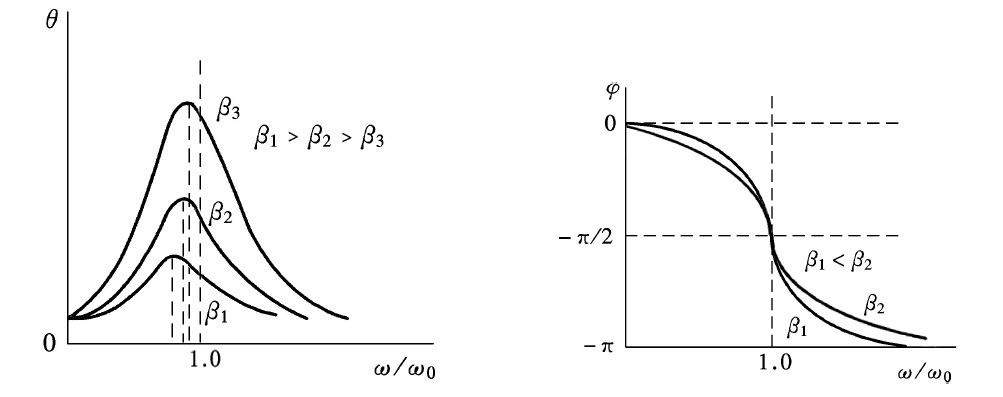
\includegraphics[width=13cm]{fig-1.png}
	\caption{The dependence of the amplitude (left) and phase shift (right) of steady-state
driven oscillations.
	\label{fig-1}}
\end{figure}

\section{Experimental setup}

The BG-2 Pohl resonator consists of two main parts: a vibrometer and a control box. The vibrometer is shown in Figure \ref{fig-2}. A copper balance wheel is mounted on a supporting frame, and the axis of the balance wheel is attached to the supporting frame with a scroll spring. The spring provides an elastic restoring torque to the wheel, which makes the balance wheel rotating about an equilibrium position.

\begin{figure}[!h]
	\centering
	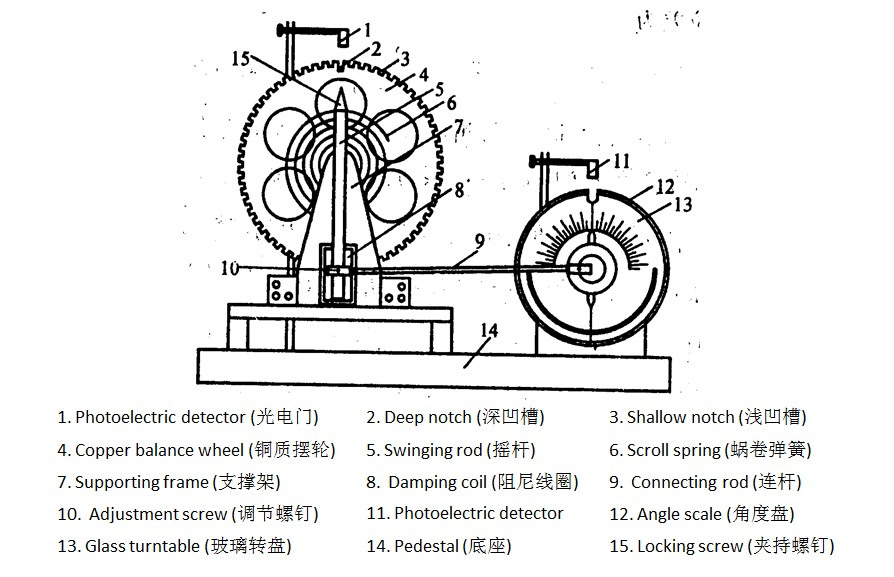
\includegraphics[width=10cm]{fig-2.png}
	\caption{The vibrometer.
	\label{fig-2}}
\end{figure}

There are many notches on the edge of the balance wheel with one notch being much deeper than the others. A photoelectric detector is set above the deep notch. The detector is used to measure the amplitude and the period of oscillations, and it is connected to the electronic control box.
\\

A pair of coils is placed at the bottom of the supporting frame, with the balance wheel fitting exactly into the gap between the two coils. Due to electromagnetic induction, the wheel will be acted upon an electromagnetic damping force when the coils are carrying current, and the magnitude of the damping force can be controlled by changing the current.
\\

The device is equipped with a motor with an eccentric wheel and a rod used to drive the wheel.
\\

There is a Period Selection switch and a Period of Driving Force knob on the electric control box, which allow to control the speed of the motor precisely. Another
photoelectric detector is set above the turntable and connected to the control box to measure the period of driving force.
\\

The phase shift can be measured using the glass turntable with an angle scale and a strobe light. The strobe is controlled by the photoelectric detector above the wheel. When the deep notch passes the equilibrium position, the detector sends a signal and the strobe flashes. In a steady state, a line on the angle scale will be highlighted by the flash of the strobe and the phase difference can be read from the angle scale directly.
\\

The amplitude of oscillations is measured by counting the notches on the wheel, and this measurement is performed by a photoelectric detector with the result displayed on the electronic control box.
\\

The front panel and the rear panel of the control box are shown in Figures \ref{fig-3} and \ref{fig-4}, respectively.

\begin{figure}[!h]
	\centering
	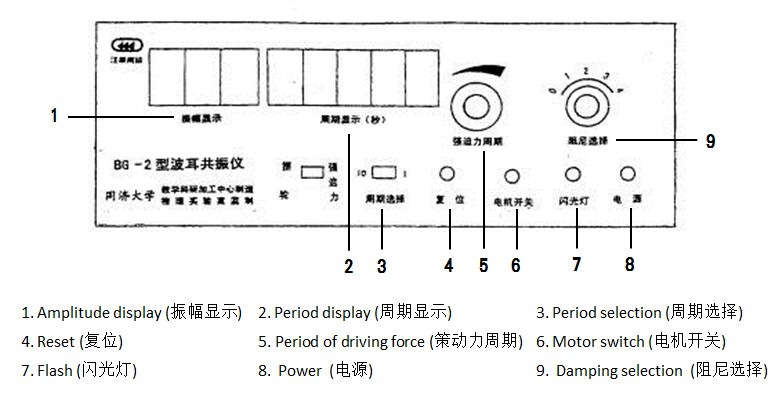
\includegraphics[width=10cm]{fig-3.png}
	\caption{The front panel of the control box.
	\label{fig-3}}
\end{figure}

The function Amplitude Display shows the oscillation amplitude of the balance wheel and Period Display shows the oscillation period in two modes. When the Period Selection switch is at position ”1”, a single oscillation period will be displayed; when the Period Selection switch is at ”10”, the time of 10 oscillation periods will be displayed. The reset button works only when the Period Selection button is at ”10”.
\\

The period of the driving force can be changed precisely by using the Period of the driving force knob, but please pay attention that the scale on the knob is not very accurate.
\\

The Damping Selection knob changes the damping force by adjusting the electric current through the coils at the bottom of the wheel. There are six options, ranging from ”0” (no current) to ”5” (current of about 0.6 A). You will use ”2”, ”3” or ”4” in this exercise.
\\

The strobe generates a flash that allows you to read the phase difference from the angle scale directly. To protect the strobe, you should turn on the Strobe switch only when measuring the phase difference.
\\

The Motor Switch is used to control the motor. You should turn the motor off when measuring the damping coefficient and the natural angular frequency.

\begin{figure}[!h]
	\centering
	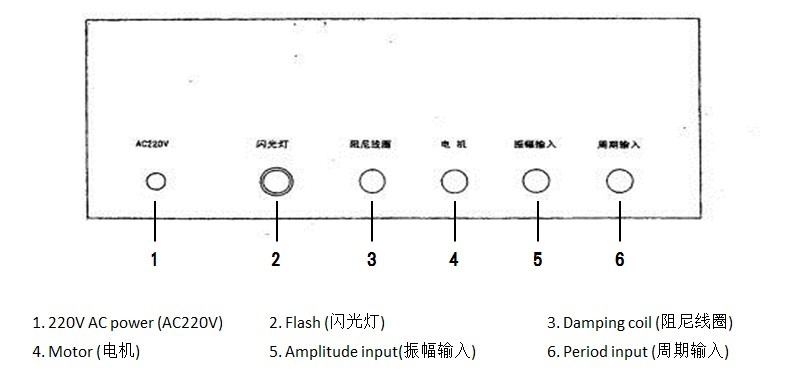
\includegraphics[width=10cm]{fig-4.png}
	\caption{The rear panel of the control box.
	\label{fig-4}}
\end{figure}

\section{Measurement}

\subsection{Measurement of Natural Angular Frequency}
\begin{enumerate}[(1)]
	\item
	Turn the Damping Selection knob to ”0”.
	\item
	Carefully rotate the balance wheel to the initial angular position $\theta_0\approx150^\circ$ and release it. Record the time of 10 periods.
	\item
	Repeat for four times and calculate the natural angular frequency $\omega_0$.
\end{enumerate}

\subsection{Measurement of Damping Coefficient}
\begin{enumerate}[(1)]
	\item
	Turn the Damping Selection knob to ”2”, and the selection should not be changed during this part.
	\item
	Carefully rotate the balance wheel to the initial amplitude of approximately $150^\circ$ and release it. Record the amplitude of each period (start from the second amplitude after you release the wheel) and the time of 10 periods.
	\item
	The solution to the homogeneous equation of motion \ref{eq-2}, with the corresponding initial conditions, is $ \theta(t)=\theta_0e^{-\beta t}cos(\omega_f t+\alpha) $. Hence $ \theta_1=\theta_0e^{-\beta T}, \theta_2=\theta_0e^{-\beta 2T},\cdots, \theta_n=\theta_0e^{-\beta nT} $. The damping coefficient $ \beta $ can then be calculated as
	$$
		ln\dfrac{\theta_i}{\theta_j}=ln\dfrac{\theta_0e^{-\beta(iT)}}{\theta_0e^{-\beta(jT)}}=(j-i)\beta T
	$$
	\item The value of $ T $ should be the average period, and $ ln\frac{\theta_i}{\theta_{i+5}} $ should be obtained by the successive difference method as
	$$\beta=\dfrac{1}{5T}ln\dfrac{\theta_i}{\theta_{i+5}}$$
\end{enumerate}

\subsection{$ \theta_{st} $ vs. $ \omega $ and $ \varphi $ vs. $ \omega $ Characteristics of Forced Oscillations}
\begin{enumerate}
	\item Keep the Damping Selection at "2", and set the speed of the motor (record the position of the motor knob in case you need to repeat the measurement). Record the amplitude $ \theta_{st} $, the period $ T $, and the phase shift $ \varphi $ when the oscillation reaches	a steady state.
	\item Repeat the steps above by changing the speed of the motor. It will result in a change of the phase shift $ \varphi $ (referred to as $ \Delta \varphi $). To make your plots more accurate, you should collect more data when $ \varphi $ and $ \theta_{st} $ change rapidly (e.g. near to the resonance point). At least 15 data should be collected for plotting.
	\item Choose Damping Selection "3". Repeat the above steps.
	\item Plot the $ \theta_{st}(\omega) $ characteristics, with $ \omega/\omega_0 $ on the horizontal axis and $ \theta_{st} $ on the
	vertical axis. Two sets of data should be plotted on the same graph.
	
	Plot the $ \varphi(\omega) $ characteristics, with $ \omega/\omega_0 $ on the horizontal axis and $ \varphi $ on the vertical
	axis. Two sets of data should be plotted on the same graph.
\end{enumerate}

\section{Results}

\subsection{Measurement of Natural Angular Frequency}

The time $10T$ through 10 periods of natural oscillations was presented in Table \ref{tab-1}.

\begin{table}[!h]
\begin{center}
\begin{tabular}{cc}
\hline
\textit{Measurement} & $10T$ [s] $\pm$ 0.001 [s] \\
\hline
1	&	15.572\\
2	&	15.575\\
3	&	15.573\\
4	&	15.577\\
\hline
\end{tabular}
\caption{Measurement of the natural frequency.}
\label{tab-1}
\end{center}
\end{table}

Then we can find the natural angular frequency

$$\omega_0=\frac{1}{4}\sum_{i=1}^4\frac{2\pi}{T_i}=4.034s^{-1}\pm1.295\times10^{-4}s^{-1}$$

\newpage

\subsection{Measurement of Damping Coefficient}

The amplitude of each period was presented in Table \ref{tab-2}.

\begin{table}[!h]
\begin{center}
\begin{tabular}{cc}
\hline
\textit{Measurement} & Amplitude [$^\circ$] $\pm$ 1 [$^\circ$] \\
\hline
$\theta_0$	&	114\\
$\theta_1$	&	103\\
$\theta_2$	&	93\\
$\theta_3$	&	85\\
$\theta_4$	&	77\\
$\theta_5$	&	70\\
$\theta_6$	&	63\\
$\theta_7$	&	57\\
$\theta_8$	&	52\\
$\theta_9$	&	47\\
\hline
\end{tabular}
\caption{Measurement of the damping coefficient.}
\label{tab-2}
\end{center}
\end{table}

Then we can simply find $k=ln(\theta_i/\theta_{i+5})$ as shown in Table \ref{tab-3}.

\begin{table}[!h]
\begin{center}
\begin{tabular}{cc}
\hline
\textit{Calculation} & $ln(\theta_i/\theta_{i+5})$ \\
\hline
1	&	0.488$\pm$0.017\\
2	&	0.492$\pm$0.019\\
3	&	0.490$\pm$0.021\\
4	&	0.491$\pm$0.023\\
5	&	0.494$\pm$0.025\\
\hline
\end{tabular}
\caption{Calculation of $ln(\theta_i/\theta_{i+5})$.}
\label{tab-3}
\end{center}
\end{table}

The average value of $ln(\theta_i/\theta_{i+5})$ was calculated based on the results presented in Table \ref{tab-3}.

$$\bar{k}=\frac{1}{5}\sum_{i=1}^5 k_i=0.491\pm0.009$$

And the time $10T$ through 10 periods of oscillations was measured as

$$10T=15.571\pm0.001s$$

Thus we can find the damping coefficient $\beta$

$$\beta=\frac{1}{5T}ln\frac{\theta_i}{\theta_{i+5}}=0.063s^{-1}\pm1.156\times10^{-3}s^{-1}$$

\newpage

\subsection{$ \theta_{st} $ vs. $ \omega $ and $ \varphi $ vs. $ \omega $ Characteristics of Forced Oscillations}

When the damping selection is 2, the results were shown in Table \ref{tab-4}.
\begin{table}[!h]
\begin{center}
\begin{tabular}{|c|c|c|c|}
\hline
\textit{Measurement} & $10T$ [s] $\pm$ 0.001 [s] &
$\varphi$ [$^\circ$] $\pm$ 1 [$^\circ$] & $\theta$ [$^\circ$] $\pm$ 1 [$^\circ$]
\\
\hline
1	&	16.532	&	-14		&	37\\
2	&	16.359	&	-17		&	43\\
3	&	16.257	&	-20		&	49\\
4	&	16.162	&	-23		&	57\\
5	&	16.067	&	-27		&	63\\
6	&	15.978	&	-32		&	73\\
7	&	15.923	&	-35.5	&	81\\
8	&	15.854	&	-41.5	&	93\\
9	&	15.809	&	-46.5	&	103\\
10	&	15.759	&	-53		&	114\\
11	&	15.679	&	-66		&	130\\
12	&	15.649	&	-71.5	&	135\\
13	&	15.576	&	-88		&	142\\
14	&	15.540	&	-96		&	142\\
15	&	15.513	&	-102.5	&	138\\
16	&	15.496	&	-106	&	136\\
17	&	15.463	&	-114	&	130\\
18	&	15.418	&	-123	&	120\\
19	&	15.375	&	-130	&	108\\
20	&	15.306	&	-139	&	91\\
21	&	15.253	&	-144	&	81\\
22	&	15.148	&	-151	&	65\\
23	&	15.069	&	-155	&	57\\
24	&	14.924	&	-161	&	43\\
25	&	14.755	&	-164	&	35\\
\hline
\end{tabular}
\caption{$ \theta_{st} $ vs. $ \omega $ and $ \varphi $ vs. $ \omega $ Characteristics.}
\label{tab-4}
\end{center}
\end{table}

\newpage

When the damping selection is 3, the results were shown in Table \ref{tab-5}.

\begin{table}[!h]
\begin{center}
\begin{tabular}{|c|c|c|c|}
\hline
\textit{Measurement} & $10T$ [s] $\pm$ 0.001 [s] &
$\varphi$ [$^\circ$] $\pm$ 1 [$^\circ$] & $\theta$ [$^\circ$] $\pm$ 1 [$^\circ$]
\\
\hline
1	&	16.459	&	-17		&	39\\
2	&	16.258	&	-22		&	49\\
3	&	16.125	&	-26		&	57\\
4	&	15.987	&	-33		&	71\\
5	&	15.908	&	-39		&	81\\
6	&	15.845	&	-45		&	91\\
7	&	15.798	&	-50		&	102\\
8	&	15.748	&	-57		&	111\\
9	&	15.711	&	-63		&	118\\
10	&	15.672	&	-69		&	123\\
11	&	15.634	&	-76		&	128\\
12	&	15.594	&	-85		&	132\\
13	&	15.551	&	-94		&	133\\
14	&	15.513	&	-102	&	130\\
15	&	15.473	&	-110	&	124\\
16	&	15.416	&	-121	&	112\\
17	&	15.350	&	-132	&	98\\
18	&	15.277	&	-139	&	83\\
19	&	15.217	&	-144	&	73\\
20	&	15.140	&	-148	&	63\\
21	&	15.053	&	-153	&	55\\
22	&	14.972	&	-156	&	47\\
23	&	14.872	&	-158	&	41\\
24	&	14.763	&	-162	&	35\\
\hline
\end{tabular}
\caption{$ \theta_{st} $ vs. $ \omega $ and $ \varphi $ vs. $ \omega $ Characteristics.}
\label{tab-5}
\end{center}
\end{table}

\begin{figure}[!p]
	\centering
	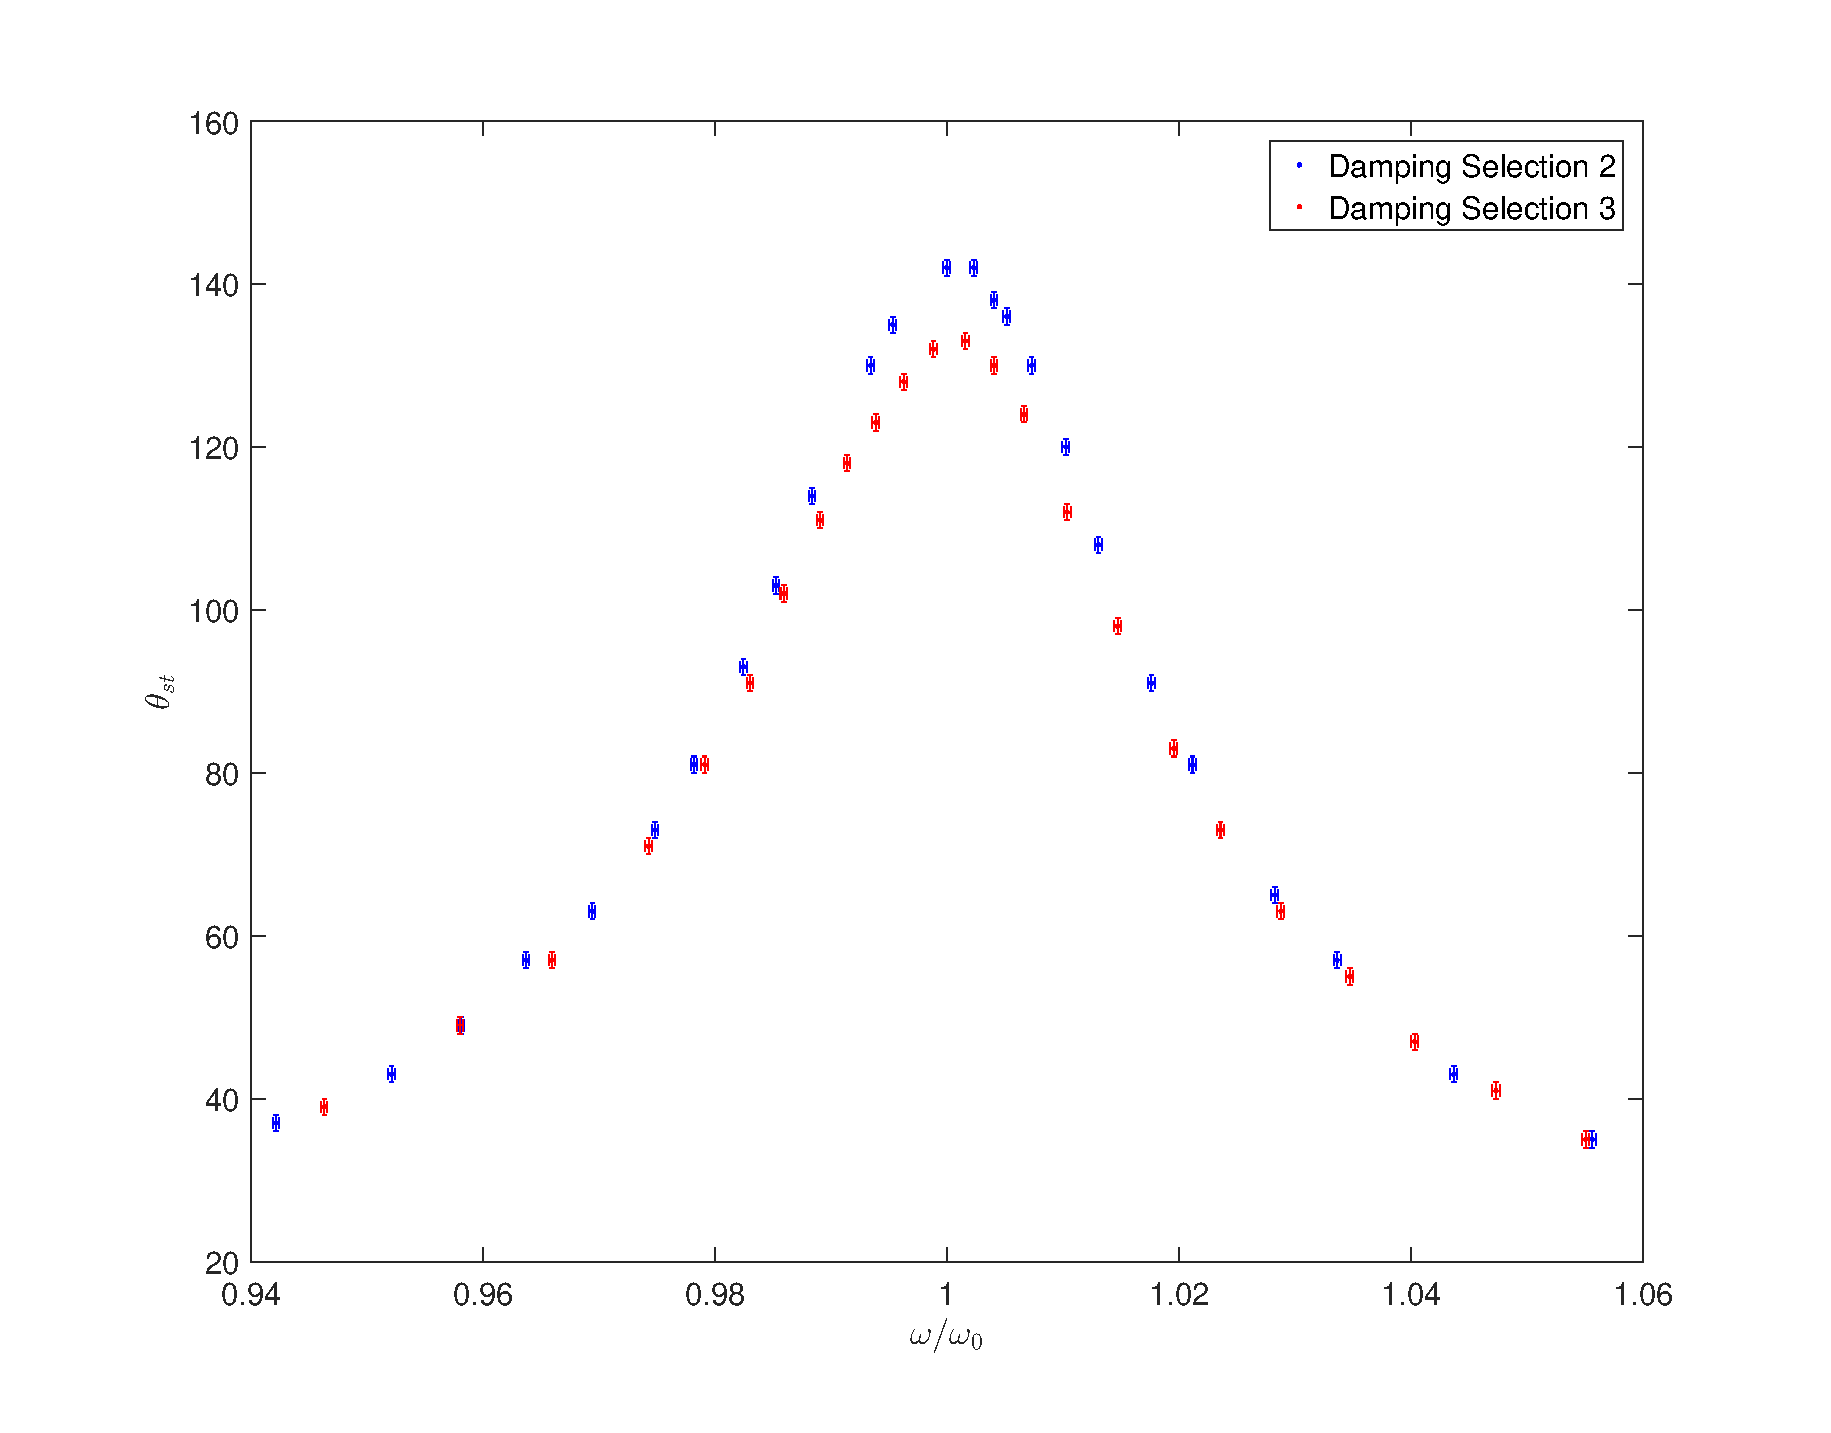
\includegraphics[width=15cm]{fig-5.eps}
	\caption{$\theta_{st}(\omega/\omega_0)$
	\label{fig-5}}
\end{figure}


\begin{figure}[!p]
	\centering
	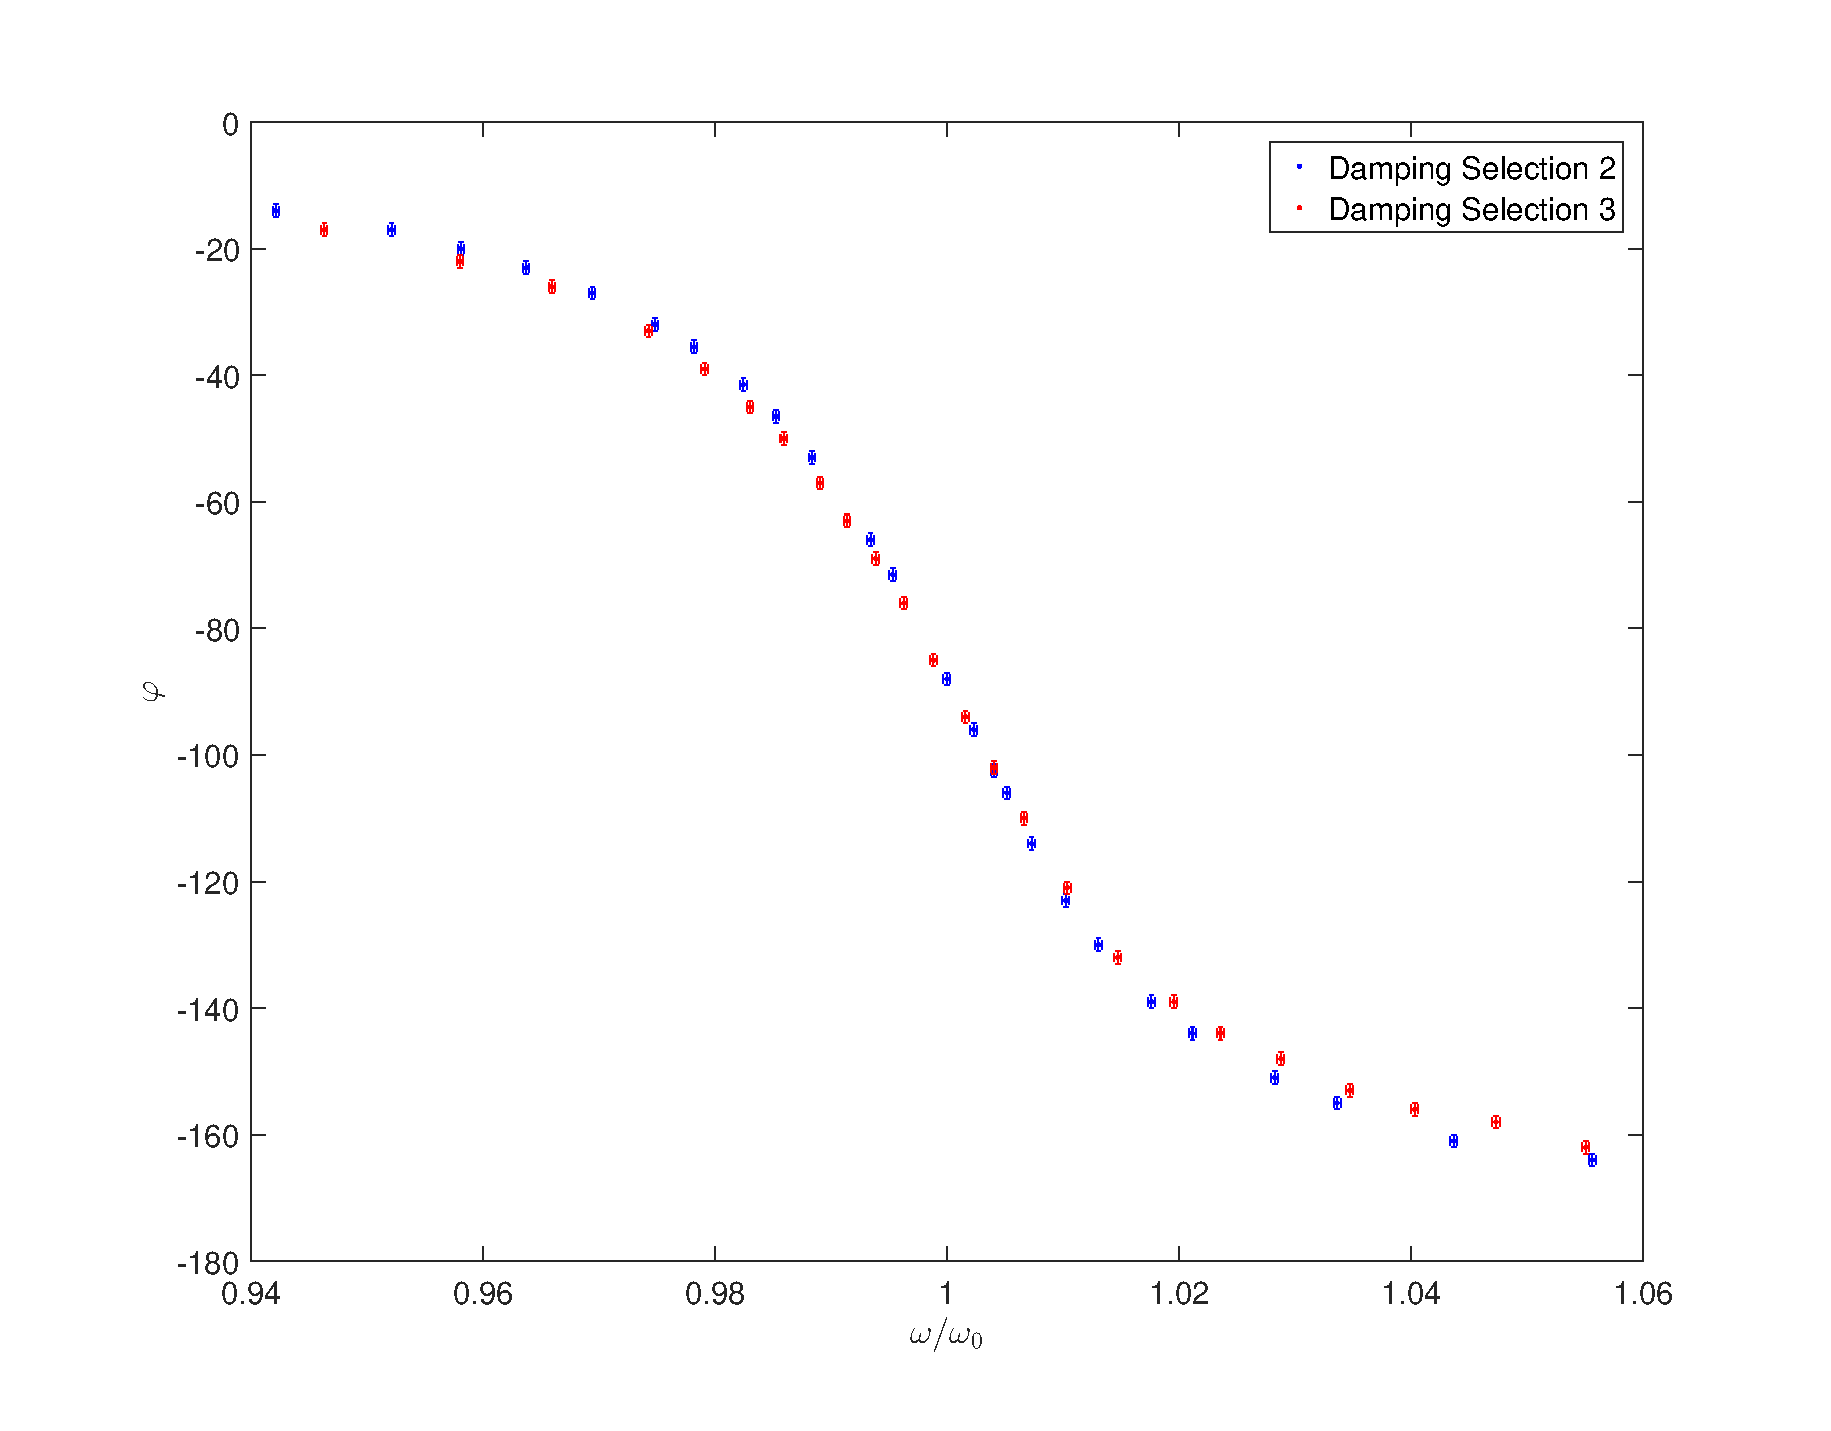
\includegraphics[width=15cm]{fig-6.eps}
	\caption{$\varphi(\omega/\omega_0)$
	\label{fig-6}}
\end{figure}

\newpage
\section{Measurement uncertainty analysis}
\subsection{Uncertainty of natural angular frequency}

The natural angular frequency can be calculated by the equation $\omega_0=\frac{2\pi}{T}$, by measuring the time of a period . Therefore its uncertainty $u_{\omega_0}$ is found by applying the uncertainty propagation formula

$$u_{\omega_0'}=\sqrt{\left[\frac{\partial}{\partial T}\left(\frac{2\pi}{T}\right)u_T\right]^2}=\frac{2\pi u_T}{T^2}$$

Given 4 uncertainties of $\omega_0$, the total uncertainty can be found by applying the uncertainty propagation formula

$$u_{\omega_0}=\frac{1}{4}\sqrt{\sum_{i=1}^4u_{\omega_{0,i}'}^2}=\frac{\pi u_T}{2}\sqrt{\sum_{i=1}^4\frac{1}{T_i^4}}=2.590\times10^{-4}$$

Hence the fixed natural angular frequency is
$$\omega_0=4.034s^{-1}\pm1.295\times10^{-4}s^{-1}$$


\subsection{Uncertainty of damping coefficient}

According to the equation $k_i=ln(\theta_i/\theta_{i+5})$, its uncertainty $u_{k_i}$ is found by applying the uncertainty propagation formula

$$u_{k_i}=\sqrt{\left(\frac{\partial k_i}{\partial\theta_i}\right)^2u_\theta^2+\left(\frac{\partial k_i}{\partial\theta_{i+5}}\right)^2u_\theta^2}
=\sqrt{\frac{1}{\theta_i^2}+\frac{1}{\theta_{i+5}^2}}$$
$$u_{k_0}=0.017,\quad u_{k_1}=0.019,\quad u_{k_2}=0.021,\quad u_{k_3}=0.023,\quad u_{k_4}=0.025$$

Given 5 uncertainties of $k$, the total uncertainty can be found by applying the uncertainty propagation formula

$$u_{k}=\frac{1}{5}\sqrt{\sum_{i=1}^4u_{k_i}^2}=0.009$$

The damping coefficient can be calculated by the equation $\beta=\frac{1}{5T}ln\frac{\theta_i}{\theta_{i+5}}=\frac{k}{5T}$, its uncertainty $u_{\beta}$ is found by applying the uncertainty propagation formula

$$u_{\beta}=\sqrt{\left(\frac{\partial \beta_i}{\partial k}\right)^2u_k^2+\left(\frac{\partial \beta_i}{\partial T}\right)^2u_T^2}
=\sqrt{\frac{u_k^2}{25T^2}+\frac{k^2u_T^2}{25T^4}}=1.156\times10^{-3}$$

Hence the fixed damping coefficient is
$$\beta=\frac{1}{5T}ln\frac{\theta_i}{\theta_{i+5}}=0.063s^{-1}\pm1.156\times10^{-3}s^{-1}$$

\newpage

\subsection{Uncertainty of $\bm{\omega/\omega_0}$}

As shown in 5.1
$$\omega=\frac{2\pi}{T}$$
$$u_{\omega}=\frac{2\pi u_T}{T^2}$$

The uncertainty of $\omega/\omega_0$ is found by applying the uncertainty propagation formula

$$u_{\omega/\omega_0}=\sqrt{\left(\frac{\partial\omega/\omega_0}{\partial\omega}\right)^2u_\omega^2+\left(\frac{\partial\omega/\omega_0}{\partial\omega_0}\right)^2u_{\omega_0}^2}
=\sqrt{\frac{u_\omega^2}{\omega_0^2}+\frac{\omega^2u_{\omega_0}^2}{\omega_0^4}}
=\frac{2\pi}{T^2\omega_0}\sqrt{u_T^2\omega_0^2+T^2u_{\omega_0}^2}$$

We can use the formula to find $u_{\omega/\omega_0}$ of all data in Table \ref{tab-4} and \ref{tab-5}, which was shown in Table \ref{tab-6}.

\begin{table}[!h]
\begin{center}
\begin{tabular}{|c|c|c|c|c|c|}
\hline
\textit{Measurement} & $\omega/\omega_0$ & Uncertainty & 
Measurement & $\omega/\omega_0$ & Uncertainty 
\\
\hline
1	&	0.942	&	2.603$\times10^{-4}$	&	1	&	0.946	&	2.623$\times10^{-4}$\\
2	&	0.952	&	2.652$\times10^{-4}$	&	2	&	0.958	&	2.681$\times10^{-4}$\\
3	&	0.958	&	2.682$\times10^{-4}$	&	3	&	0.966	&	2.721$\times10^{-4}$\\
4	&	0.964	&	2.710$\times10^{-4}$	&	4	&	0.974	&	2.763$\times10^{-4}$\\
5	&	0.969	&	2.739$\times10^{-4}$	&	5	&	0.979	&	2.788$\times10^{-4}$\\
6	&	0.975	&	2.766$\times10^{-4}$	&	6	&	0.983	&	2.808$\times10^{-4}$\\
7	&	0.978	&	2.783$\times10^{-4}$	&	7	&	0.986	&	2.823$\times10^{-4}$\\
8	&	0.982	&	2.805$\times10^{-4}$	&	8	&	0.989	&	2.839$\times10^{-4}$\\
9	&	0.985	&	2.819$\times10^{-4}$	&	9	&	0.991	&	2.851$\times10^{-4}$\\
10	&	0.988	&	2.835$\times10^{-4}$	&	10	&	0.994	&	2.864$\times10^{-4}$\\
11	&	0.993	&	2.861$\times10^{-4}$	&	11	&	0.996	&	2.876$\times10^{-4}$\\
12	&	0.995	&	2.871$\times10^{-4}$	&	12	&	0.999	&	2.890$\times10^{-4}$\\
13	&	1.000	&	2.896$\times10^{-4}$	&	13	&	1.002	&	2.904$\times10^{-4}$\\
14	&	1.002	&	2.908$\times10^{-4}$	&	14	&	1.004	&	2.917$\times10^{-4}$\\
15	&	1.004	&	2.917$\times10^{-4}$	&	15	&	1.007	&	2.930$\times10^{-4}$\\
16	&	1.005	&	2.922$\times10^{-4}$	&	16	&	1.010	&	2.950$\times10^{-4}$\\
17	&	1.007	&	2.934$\times10^{-4}$	&	17	&	1.015	&	2.973$\times10^{-4}$\\
18	&	1.010	&	2.949$\times10^{-4}$	&	18	&	1.020	&	2.999$\times10^{-4}$\\
19	&	1.013	&	2.964$\times10^{-4}$	&	19	&	1.024	&	3.020$\times10^{-4}$\\
20	&	1.018	&	2.988$\times10^{-4}$	&	20	&	1.029	&	3.048$\times10^{-4}$\\
21	&	1.021	&	3.007$\times10^{-4}$	&	21	&	1.035	&	3.080$\times10^{-4}$\\
22	&	1.028	&	3.045$\times10^{-4}$	&	22	&	1.040	&	3.110$\times10^{-4}$\\
23	&	1.034	&	3.074$\times10^{-4}$	&	23	&	1.047	&	3.148$\times10^{-4}$\\
24	&	1.044	&	3.128$\times10^{-4}$	&	24	&	1.055	&	3.190$\times10^{-4}$\\
25	&	1.056	&	3.193$\times10^{-4}$	&		&			&\\
\hline
\end{tabular}
\caption{Uncertainty of $u_{\omega/\omega_0}$.}
\label{tab-6}
\end{center}
\end{table}


\newpage
\section{Conclusion}

In the experiment, we studied damped and driven oscillations in mechanical systems using the Pohl resonator.
\\

In order to to get the time $T$  of a period of oscillation, we measured 10$T$ each time and divided it by 10 to improve its accuracy. Then we can get the angular frequency by the formula

$$\omega_0=\frac{2\pi}{T}$$

When calculating the damping coefficient $\beta$, we measured 10 continuous amplitude of the damping and then used the formula

$$\beta=\dfrac{1}{5T}ln\dfrac{\theta_i}{\theta_{i+5}}$$

It was necessary to get two $\theta$s at a distance of 5 in order to make the experiment more accurate. It was successful because the final uncertainty of $\beta$ is $1.156\times10^{-3}s^{-1}$, which is relative small according to the value of $\beta=0.063s^{-1}$
\\

Finally, we found the relationship between $\theta_{st},\ \varphi$ and $\omega/\omega_0$ under different selections of damping. 

After plot two of the selected damping, we can find that they were similar to the theorem. The comparison was shown in Figure \ref{fig-7}.
\\

The curves in the curve seemed smooth and the uncertainty of the curve was very small, which suggested that the experiment was done successfully and satisfied the two formulas

$$\theta_{st}=\frac{\mu}{\sqrt{(\omega_0^2-\omega^2)^2+4\beta^2\omega^2}}$$

$$\tan\varphi=\frac{2\beta\omega}{\omega^2-\omega_0^2}$$

However, the equipment in the lab was old so that we had to wait much time until the result became stable, which made the experiment time longer than we expected. If this could be improved, the experiment will become more friendly to us.

\begin{figure}[h!]
	\centering
	\subfigure[$\theta_{st}$]{
	\label{Fig.sub.1}
	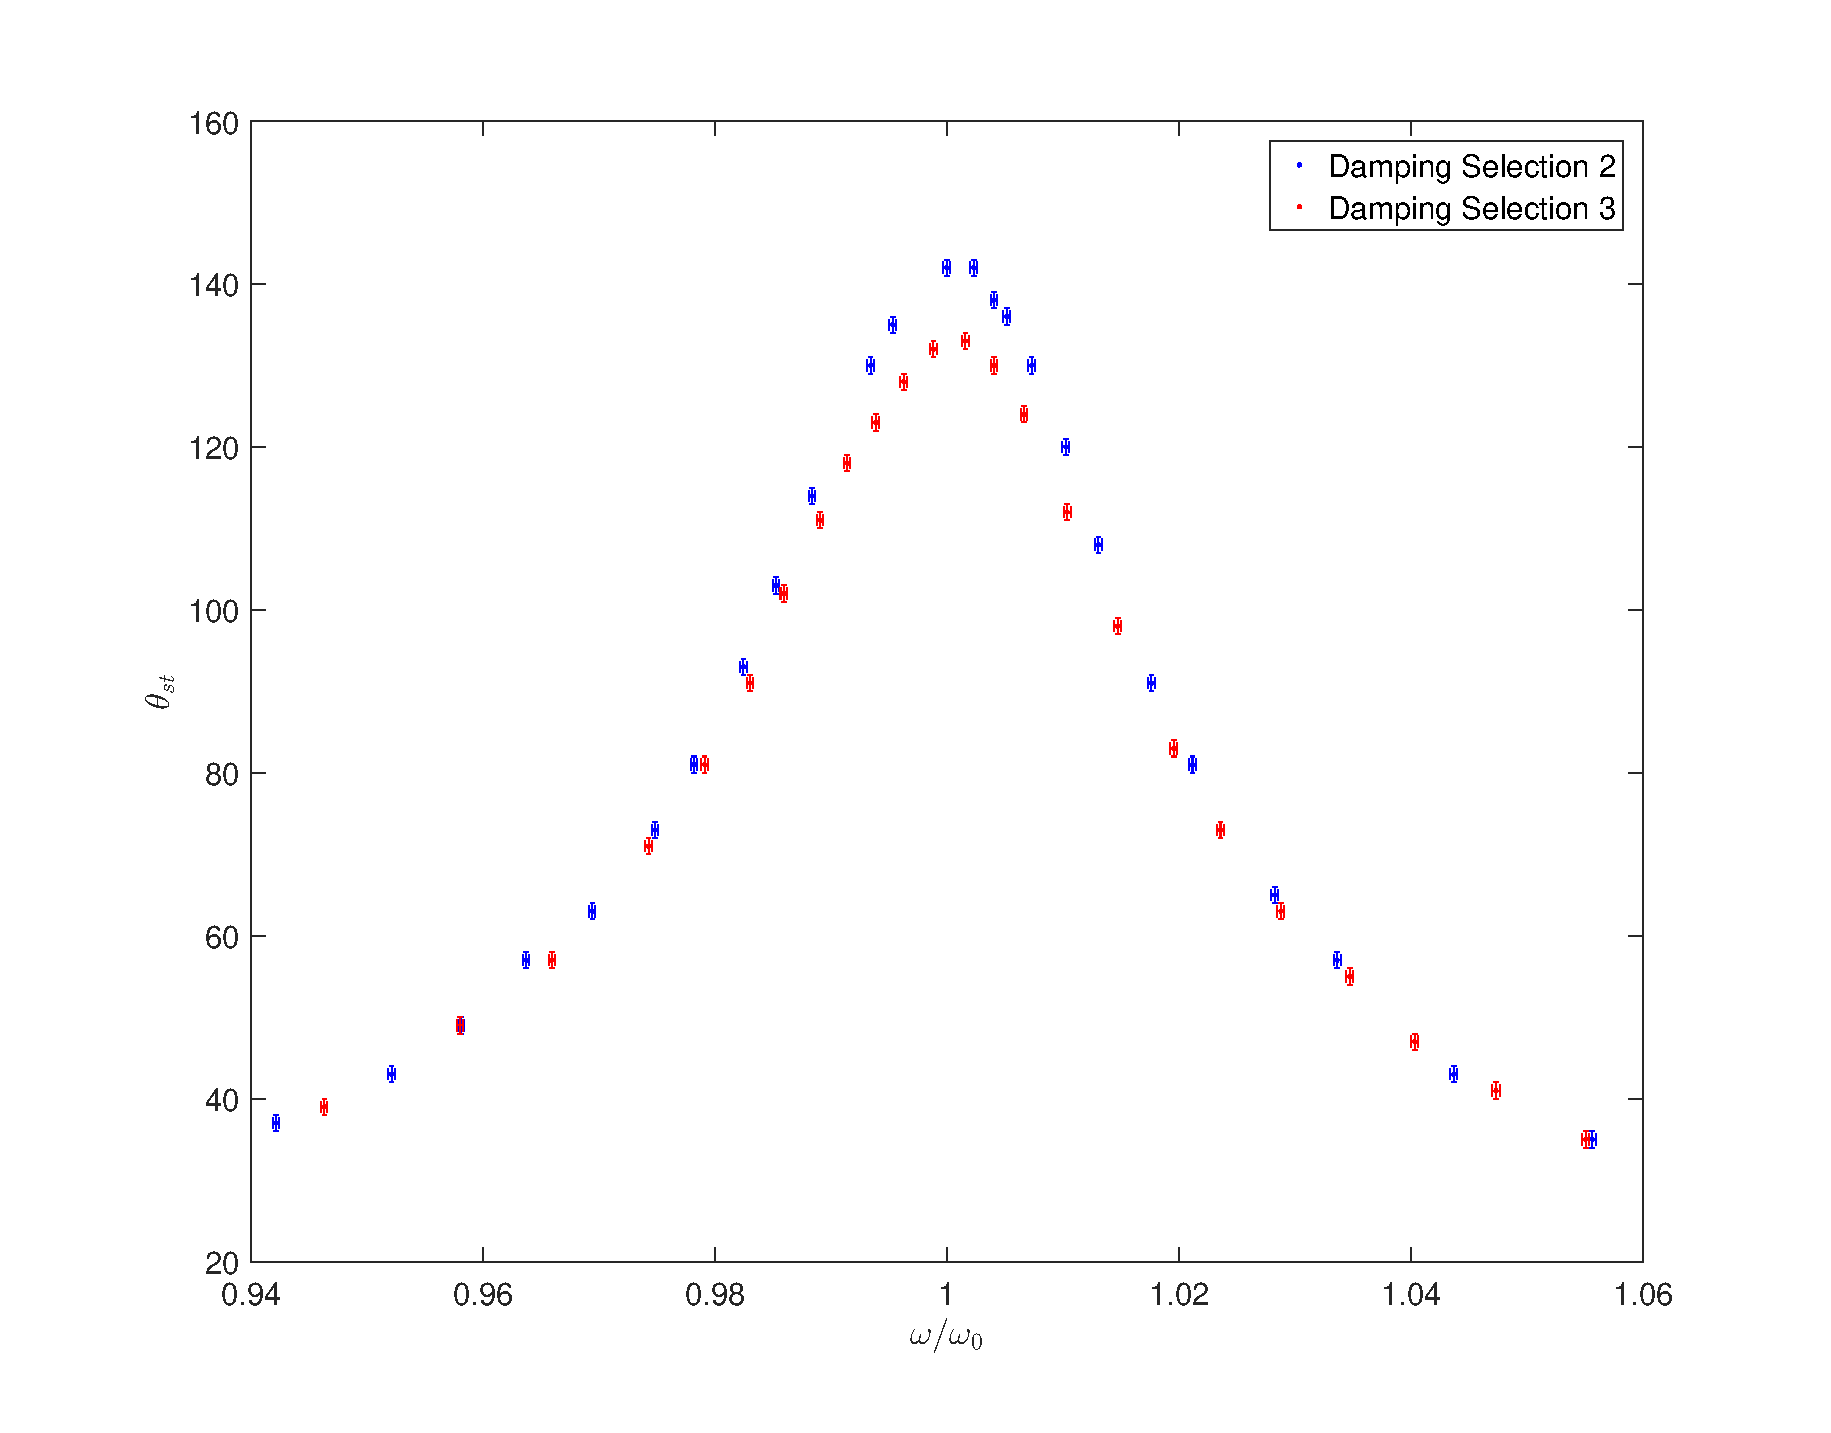
\includegraphics[width=7cm]{fig-5.eps}}
	\subfigure[$\varphi$]{
	\label{Fig.sub.2}
	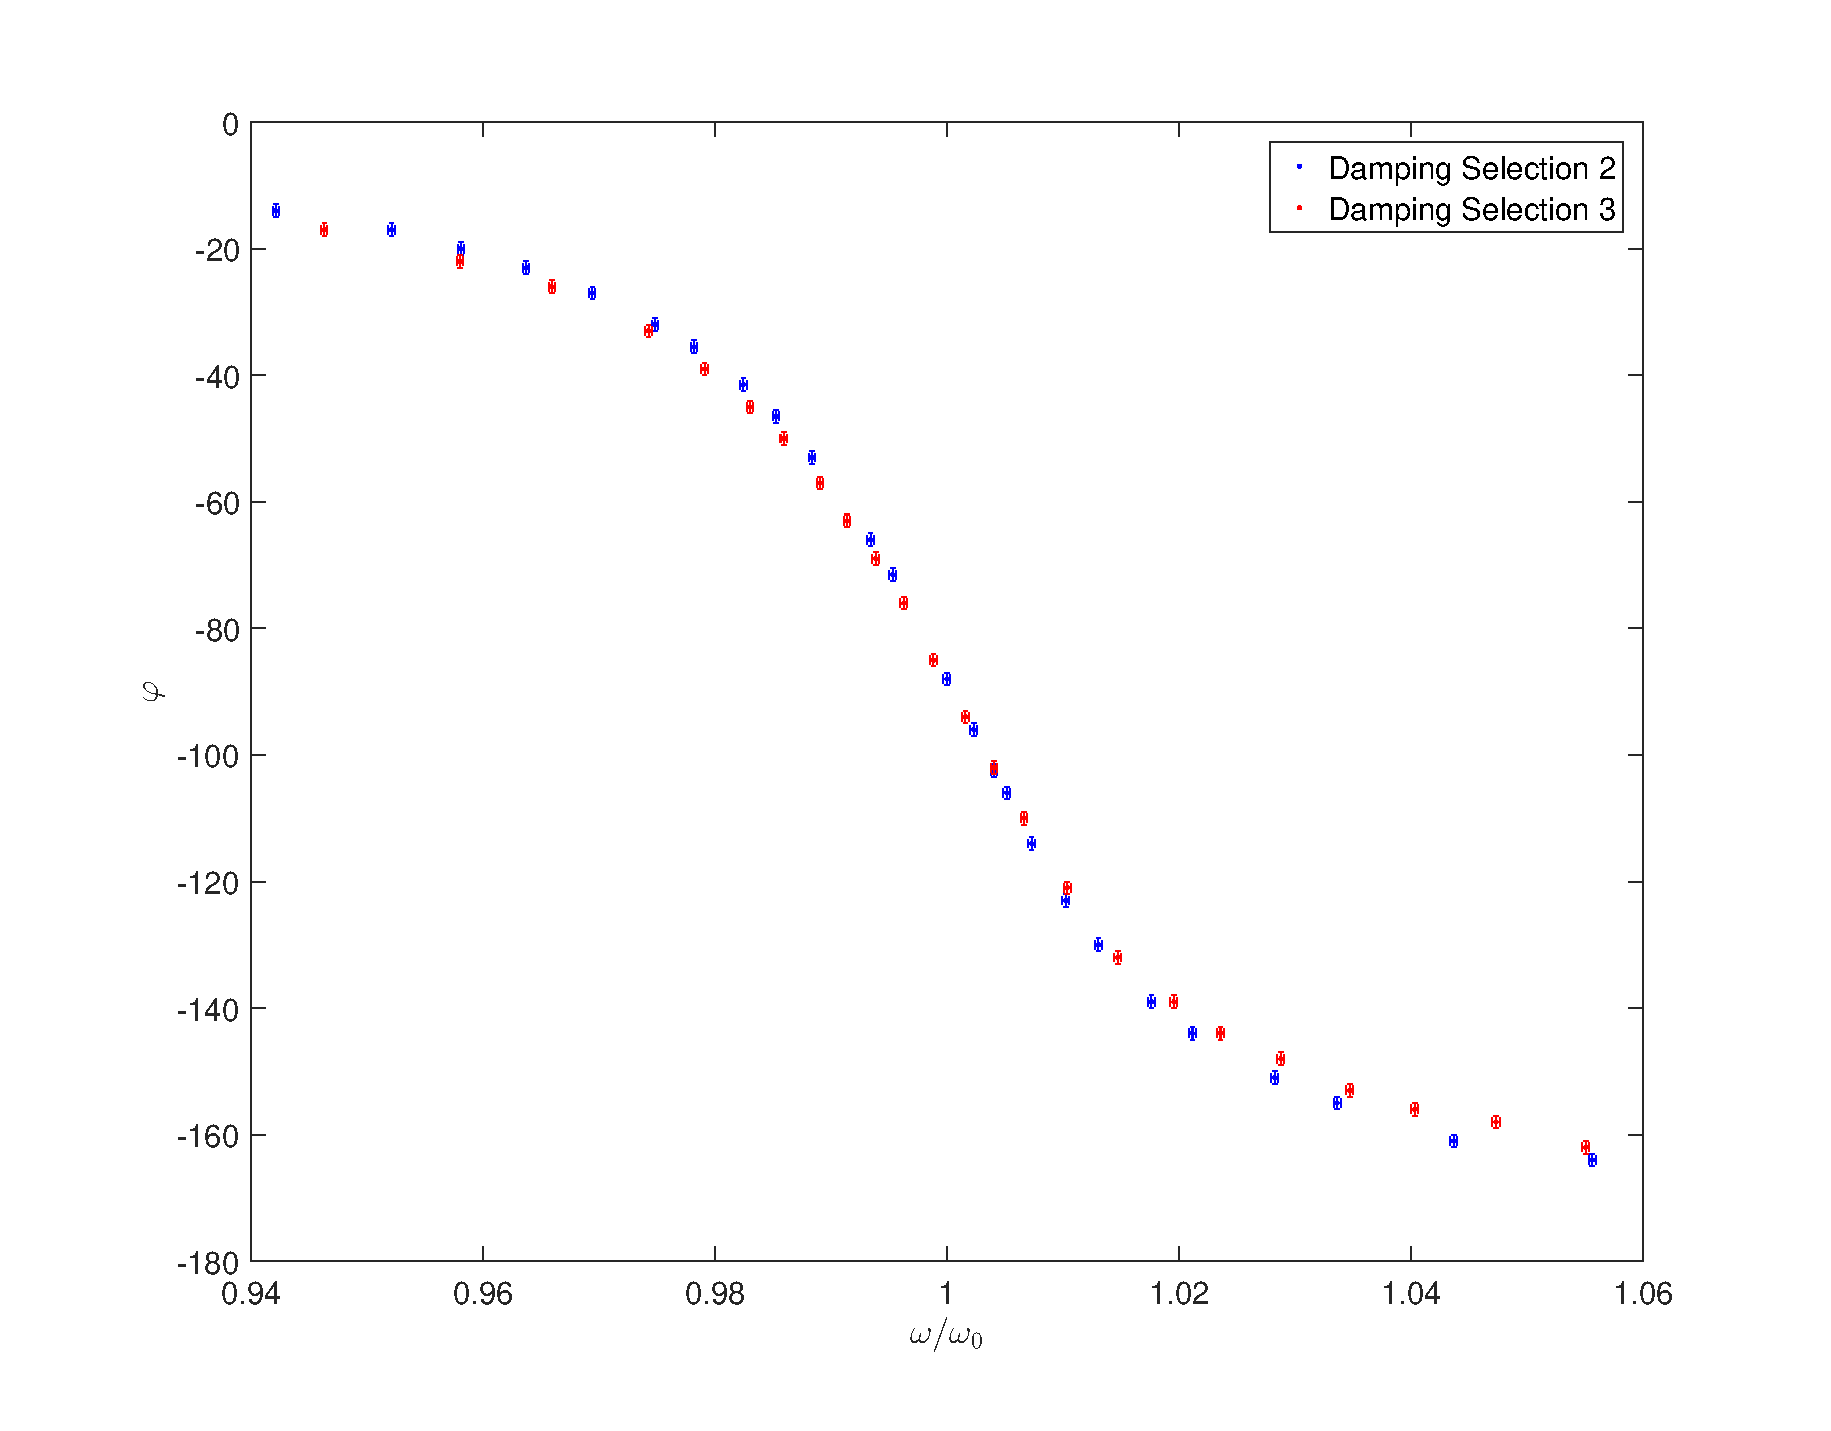
\includegraphics[width=7cm]{fig-6.eps}}
	\subfigure[theorem]{
	\label{Fig.sub.3}
	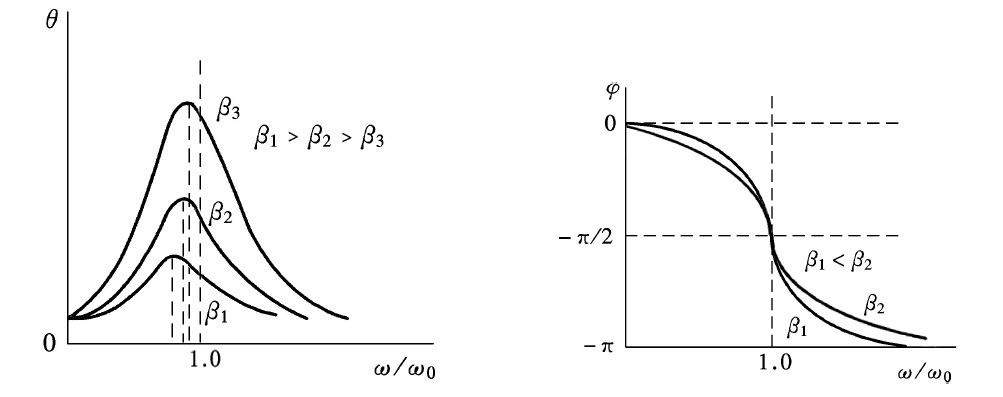
\includegraphics[width=15cm]{fig-1.png}}
	\caption{Comparison between the result and theorem.}
	\label{fig-7}
\end{figure}

\section{Reference}

\begin{enumerate}[(a)]
	\item
	Qin Tian, Wang Yin, Mateusz Krzyzosiak, VP141 Exercise 5, Damped and Driven Oscillations. Mechanical Resonance, based on materials provided by the Department of Physics, Shanghai Jiaotong University.
\end{enumerate}

\end{document}